% Auto-generated MATLAB pure-vs-MEX comparison.
\begin{center}\small
\begin{longtable}{@{}lrr rr rr r@{}}
\toprule
\textbf{Case} & \textbf{Buses} & \textbf{Sol.} & \textbf{pure wall} & \textbf{MEX wall} & \textbf{pure} & \textbf{MEX} & \textbf{MEX}\\
 & & & \multicolumn{2}{c}{\emph{search wall (s)}} & \multicolumn{2}{c}{\emph{ms/trace}} & \textbf{$\times$}\\
\midrule\endhead
\code{case3} & 3 & 6 & 0.5 & 0.3 & 119 & 68.1 & 1.75\\
\code{case3TS} & 3 & 6 & 0.2 & 0.1 & 53.4 & 23.0 & 2.33\\
\code{case4gs} & 4 & 4 & 0.3 & 0.2 & 69.8 & 34.1 & 2.05\\
\code{case7Salam} & 7 & 4 & 0.3 & 0.2 & 90.3 & 39.5 & 2.29\\
\code{case6ww} & 6 & 6 & 0.4 & 0.2 & 74.5 & 33.6 & 2.22\\
\code{case9} & 9 & 8 & 0.7 & 0.3 & 118 & 54.0 & 2.18\\
\code{case9Q} & 9 & 8 & 0.5 & 0.3 & 100 & 46.6 & 2.15\\
\code{case4BBc} & 4 & 12 & 0.3 & 0.6 & 63.5 & 44.4 & 1.43\\
\code{case4BB0} & 4 & 14 & 0.5 & 0.3 & 84.3 & 43.3 & 1.95\\
\code{case5loop} & 5 & 10 & 0.6 & 0.3 & 69.3 & 29.3 & 2.36\\
\code{case5Salam} & 5 & 10 & 0.6 & 0.5 & 97.5 & 77.3 & 1.26\\
\code{case5Salam\_mod3} & 5 & 4 & 0.2 & 0.2 & 61.1 & 48.5 & 1.26\\
\code{case14mod} & 14 & 30 & 3.1 & 2.2 & 168 & 116 & 1.46\\
\code{case14mod2} & 14 & 68 & 5.3 & 3.8 & 143 & 82.2 & 1.74\\
\code{case33bw} & 33 & 16 & 7.0 & 3.4 & 247 & 113 & 2.19\\
\code{case39} & 39 & 176 & 50.7 & 28.0 & 200 & 93.2 & 2.15\\
\code{case30} & 30 & 472 & 85.0 & 48.8 & 159 & 72.6 & 2.19\\
\code{case\_ieee30} & 30 & 472 & 88.1 & 48.6 & 167 & 72.0 & 2.31\\
\code{case57mod} & 57 & 606 & 293 & 139 & 212 & 80.2 & 2.64\\
\code{case57} & 57 & 1322 & 608 & 309 & 222 & 91.8 & 2.42\\
\bottomrule
\end{longtable}
\end{center}

\textbf{Summary.} The pure-MATLAB and MEX builds return identical solution counts on every case (3,254 solutions in total). From the rounded table, summed search wall time is 1,145.3~s for pure MATLAB and 586.3~s for MEX (1.95$\times$ aggregate); the geometric-mean case-wise wall factor is 1.59$\times$. The compiled MEX hot path (KLU corrector, Pad\'e and holomorphic kernels) speeds up the numerical kernel per trace by a geometric-mean factor of 1.97$\times$. The preserved table does not include per-solution residual vectors, so it supports no new residual-distance claim.

\IfFileExists{matlab_benchmark.png}{%
\begin{center}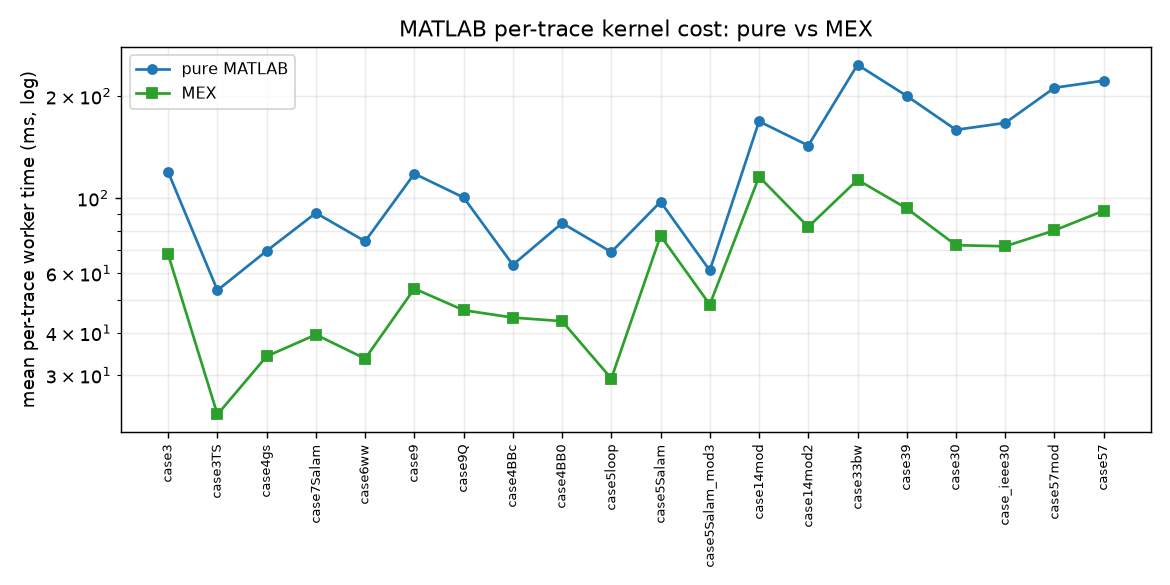
\includegraphics[width=0.72\textwidth]{matlab_benchmark.png}\end{center}}{}
